\documentclass[letterpaper,headings=standardclasses]{scrartcl}

\usepackage[margin=1in,includefoot]{geometry}
\usepackage{amssymb}
\usepackage{amsmath}
\usepackage{listings}
\usepackage{tikz}
\usepackage{float}
\usepackage{algorithm}
\usepackage{algpseudocode}

\usetikzlibrary{shapes,arrows}

\tikzset{
  block/.style    = {draw, thick, rectangle, minimum height = 3em, minimum width = 3em},
  sum/.style      = {draw, circle},
  input/.style    = {coordinate, circle},
  output/.style   = {coordinate, circle}
}

\lstset{basicstyle=\ttfamily,language=python,columns=flexible,breaklines=true,showstringspaces=false}

\title{Homework 4}
\subtitle{CS 559 - Neural Networks - Fall 2019}
\author{Matteo Corain 650088272}

\begin{document}

\maketitle

\section{Question 1}

\subsection{Training set generation}

According to the specifications of the exercise, the training set for the considered neural network has been generated as a set of 300 unidimensional samples $x_i, i = 1, \dots, 300$, drawn at random in $[0, 1]$; this was accomplished by means of the \texttt{uniform()} function provided by the NumPy library and the obtained samples were stored in the \texttt{x} array. A set of noise samples $\nu_i$ was also created, by drawing at random some values in $\left[-\frac{1}{10},\frac{1}{10}\right]$ and storing them in array \texttt{n}. Starting from these two arrays, the expected outputs have been generated by means of the function that the considered network needs to approximate, expressed using the functions provided by the NumPy library and stored in the array \texttt{d}:

$$ d_i = \text{sin}(20x_i) + 3x_i + \nu_i $$

\subsection{Feed-forward procedure}

The backpropagation training algorithm has been implemented using the matricial form presented in class. Specifically, let us consider a network with $L \ge 1 $ layers, indicating as $m_i$ the number of neurons in the $i$-th layer. Each layer $i$ of the network receives an input $y_{i - 1}$ and produces an output $y_i$ by applying its activation function $\phi_i (v_i)$ to its induced field $v_i = W_i \left[ \begin{matrix} 1 & y_{i - 1} \end{matrix} \right]^T$, where $W_i$ is the weight matrix of the $i$-th layer.

The feedforward phase of the algorithm may therefore be implemented by repeating $L$ times (one for each layer) the following operations:

\begin{itemize}
    \item Compute the local induced field:
    $$ v_i = W_i \left[ \begin{matrix} 1 \\ y_{i - 1} \end{matrix} \right] $$
    \item Compute the layer output:
    $$ y_i = \phi_i (v_i) $$
\end{itemize}

For the first layer of the network, the input $y_0$ is the input $x$ of the network. The feedforward procedure may be implemented using algorithm \ref{ffalg}.

\begin{algorithm}[h]
    \caption{Feed-forward procedure}
    \label{ffalg}
    \begin{algorithmic}
    
    \Function{Feed-Forward}{$x_i, W, \phi$}
        \State \Comment{Initialization}
        \State $v \gets $ \Call{Empty-List}{}
        \State $y \gets $ \Call{Empty-List}{}
        \State $y[0] \gets x_i$
        \State \Comment{Computation of $v$ and $y$ values}
        \For{$i = 1, \dots, L$}
            \State $v[i] \gets W[i] \left[ \begin{matrix} 1 & y[i] \end{matrix} \right]^T$
            \State $y[i + 1] \gets \phi[i](v[i])$
        \EndFor
        \State \Return $v, y$
    \EndFunction
    
    \end{algorithmic}
\end{algorithm}

\subsection{Backpropagation procedure}

The partial results coming from the $v$ and $y$ vectors can then be used to compute the update terms for the gradient descent algorithm (to be precise, to estimate the value of the derivatives $\frac{\partial E}{\partial W_i}, \forall i$). Let us define the quantities $\delta_i, i = 1, \dots, L$ as:

$$ \delta_i = \begin{cases} (d - y_L) \cdot \phi'(v_L) & \text{if } i = L \\ \left( W^*_{i + 1} \right)^T \delta_{i + 1} \cdot \phi'(v_i) & \text{if } i = 1, \dots, L - 1 \end{cases} $$

Where the $\cdot$ symbol denotes a dot product operation and $W^*_i$ denotes the $W_i$ matrix to which the first row has been removed (the one related to the bias contributions). The theoretical results of the backpropagation algorithm prove that, once the $\delta_i$ quantities are defined, it is possible to compute the partial derivatives of $E$ as:

$$ \frac{\partial E}{\partial W_i} = - \delta_i \left[ \begin{matrix} 1 \\ y_{i - 1} \end{matrix} \right] $$

This suggests the procedure shown in algorithm \ref{bpalg} to implement the backpropagation mechanism.

\begin{algorithm}[h]
    \caption{Backpropagation procedure}
    \label{bpalg}
    \begin{algorithmic}
    
    \Function{Backpropagate}{$x_i, d, W, \phi, \phi'$}
        \State \Comment{Initialization}
        \State $v, y \gets $ \Call{Feed-Forward}{$x_i, W, \phi$}
        \State $\delta \gets $ \Call{Empty-List}{}
        \State $\nabla E \gets $ \Call{Empty-List}{}
        \State \Comment{Computation of $\delta_i$ values}
        \State $\delta[L] \gets (d - y[L]) * \phi'[L](v[L])$
        \For{$i = L - 1, \dots, 1$}
            \State $\delta[i] \gets \left( W^*[i + 1] \right)^T \delta[i + 1] * \phi'[i](v[i])$
        \EndFor
        \State \Comment{Computation of $\nabla E$ components}
        \For{$i = 1, \dots, L$}
            \State $\nabla E[i] = -\delta[i] \left[ \begin{matrix} 1 & y_{i - 1} \end{matrix} \right]^T$
        \EndFor
        \State \Return $v, y$
    \EndFunction
    
    \end{algorithmic}
\end{algorithm}

\subsection{Error procedure}

The error procedure is used to compute the value of the error function, given the current weights, the activation functions, the training samples and the associated desired outputs. Let us recall that the error function may be computed using the formula:

$$ E = \frac{1}{n} \sum_{i = 1}^{n} || d_i - y_{i,L} ||^2 $$

Where $n$ is the number of training samples ($n = 300$, in this case). Algorithm \ref{eralg} shows a possible implementation of the error procedure.

\begin{algorithm}[h]
    \caption{Error procedure}
    \label{eralg}
    \begin{algorithmic}
    
    \Function{Error}{$x, d, n, W, \phi$}
        \State $e \gets 0$
        \For{$i = 1, \dots, n$}
            \State $v, y \gets $ \Call{Feed-Forward}{$x[i], W, \phi$}
            \State $e \gets e + (d[i] - y[L])^2$
        \EndFor
        \State \Return $e / n$
    \EndFunction
    
    \end{algorithmic}
\end{algorithm}

\subsection{Training procedure}

The training procedure is the one that is effectively used to train the network, computing the update terms starting from the results of the backpropagation procedure. It implements a standard gradient descent method, in which weights are updated for each sample as:

$$ W_i \leftarrow W_i - \eta \frac{\partial E}{\partial W_i}, i = 1, \dots, L $$

In which the derivative term is computed through the backpropagation procedure. This can be implemented as shown in algorithm \ref{tralg}, which uses as stopping criteria two conditions:

\begin{itemize}
    \item The reduction of the energy function $E$ obtained after an update is lower than some $\epsilon$;
    \item The maximum number of epochs $\lambda$ has been reached.
\end{itemize}

This algorithm also implements the $\eta$ update rule, which reduces the learning rate by a factor of 0.9 when it detects that the error increases from an epoch to the next.

\begin{algorithm}[h]
    \caption{Training procedure}
    \label{tralg}
    \begin{algorithmic}
    
    \Function{Train}{$x, d, W, \phi, \phi', n, \eta, \epsilon, \lambda$}
        \State \Comment{Initialization}
        \State $epochs \gets 0$
        \State $errors \gets $ \Call{Empty-List}{}
        \State $errors[0] \gets $ \Call{Error}{$x, d, W, \phi$}
        \State \Comment{Main weights update loop}
        \While{$epochs < \lambda \vee errors[epochs - 1] - errors[epochs] > \epsilon$}
            \State $epochs \gets epochs + 1$
            \State \Comment{Compute update terms and update weights}
            \For{$i = 1, \dots, n$}
                \State $\nabla E \gets $ \Call{Backpropagate}{$x[i], d[i], W, \phi, \phi'$}
                \For{$j = 1, \dots, L$}
                    \State $W[j] \gets W[j] - \eta \nabla E[j]$
                \EndFor
            \EndFor
            \State \Comment{Error registration}
            \State $errors[epochs] \gets $ \Call{Error}{$x, d, W, \phi$}
            \State \Comment{Update of $\eta$}
            \If{$errors[epochs] > errors[epochs - 1]$}
                \State $\eta \gets 0.9 \eta$
            \EndIf
        \EndWhile
        \State \Return $v, y$
    \EndFunction
    
    \end{algorithmic}
\end{algorithm}

\subsection{Implementation details}

The described algorithms were implemented using the Python programming language in conjunction with the NumPy scientific computing library. In particular, we have that:

\begin{itemize}
    \item Procedure \textsc{Feed-Forward} is implemented in the \texttt{feedforward()} function;
    \item Procedure \textsc{Backpropagate} is implemented in the \texttt{backpropagate()} function;
    \item Procedure \textsc{Error} is implemented in the \texttt{error()} function;
    \item Procedure \textsc{Train} is implemented in the \texttt{train()} function.
\end{itemize}

The initial weights matrices \texttt{W1} and \texttt{W2} for the network have been chosen according to the weight initialization heuristic, which prescribes to draw the starting values from a normal distribution, with mean $\mu = 0$ and variance $\sigma^2 = \frac{1}{m}$, where $m$ is the number of neurons in the network. In the considered case, we have $m = 25$, so a reasonable value for the standard deviation could be $\sigma = 0.2$. As for the training parameters, the following values have been chosen:

$$ \eta = 0.1, \epsilon = 10^{-9}, \lambda = 100000 $$

The training procedure has then been executed, using as parameters:

\begin{itemize}
    \item The \texttt{x} and \texttt{d} vectors generated as explained before;
    \item The lists \texttt{W = [W1, W2]}, \texttt{phi = [phi1, phi2]} and \texttt{der\_phi = [der\_phi1, der\_phi2]}, containing respectively the two weight matrices, the two activation functions and their two derivatives (passed as function pointers);
    \item The three training parameters \texttt{eta = 0.1}, \texttt{eps = 1e-9} and \texttt{lambda = 100000}.
\end{itemize}

\subsection{Results}

The training algorithm was able to converge to a good enough fit in 47520 epochs, at the end of which the value of the error function is about:

$$ E = 0.00521 $$

Results have been plotted by making use of the \texttt{plot\_fit()} and \texttt{plot\_errors()} functions. The first is used to plot the function fitted from the generated dataset, obtained by evaluating the output of the network (through the \texttt{feedforward()} function) on a evenly-spaced set of $x$ values (generated using the \texttt{linspace()} function of the NumPy library). The second simply plots the contents of the passed \texttt{errors} list for increasing number of epochs.

The obtained fitting is shown in figure \ref{fit_9}; figure \ref{err_9} shows instead the value of the error function for increasing epochs.

\begin{figure}[h]
\centering
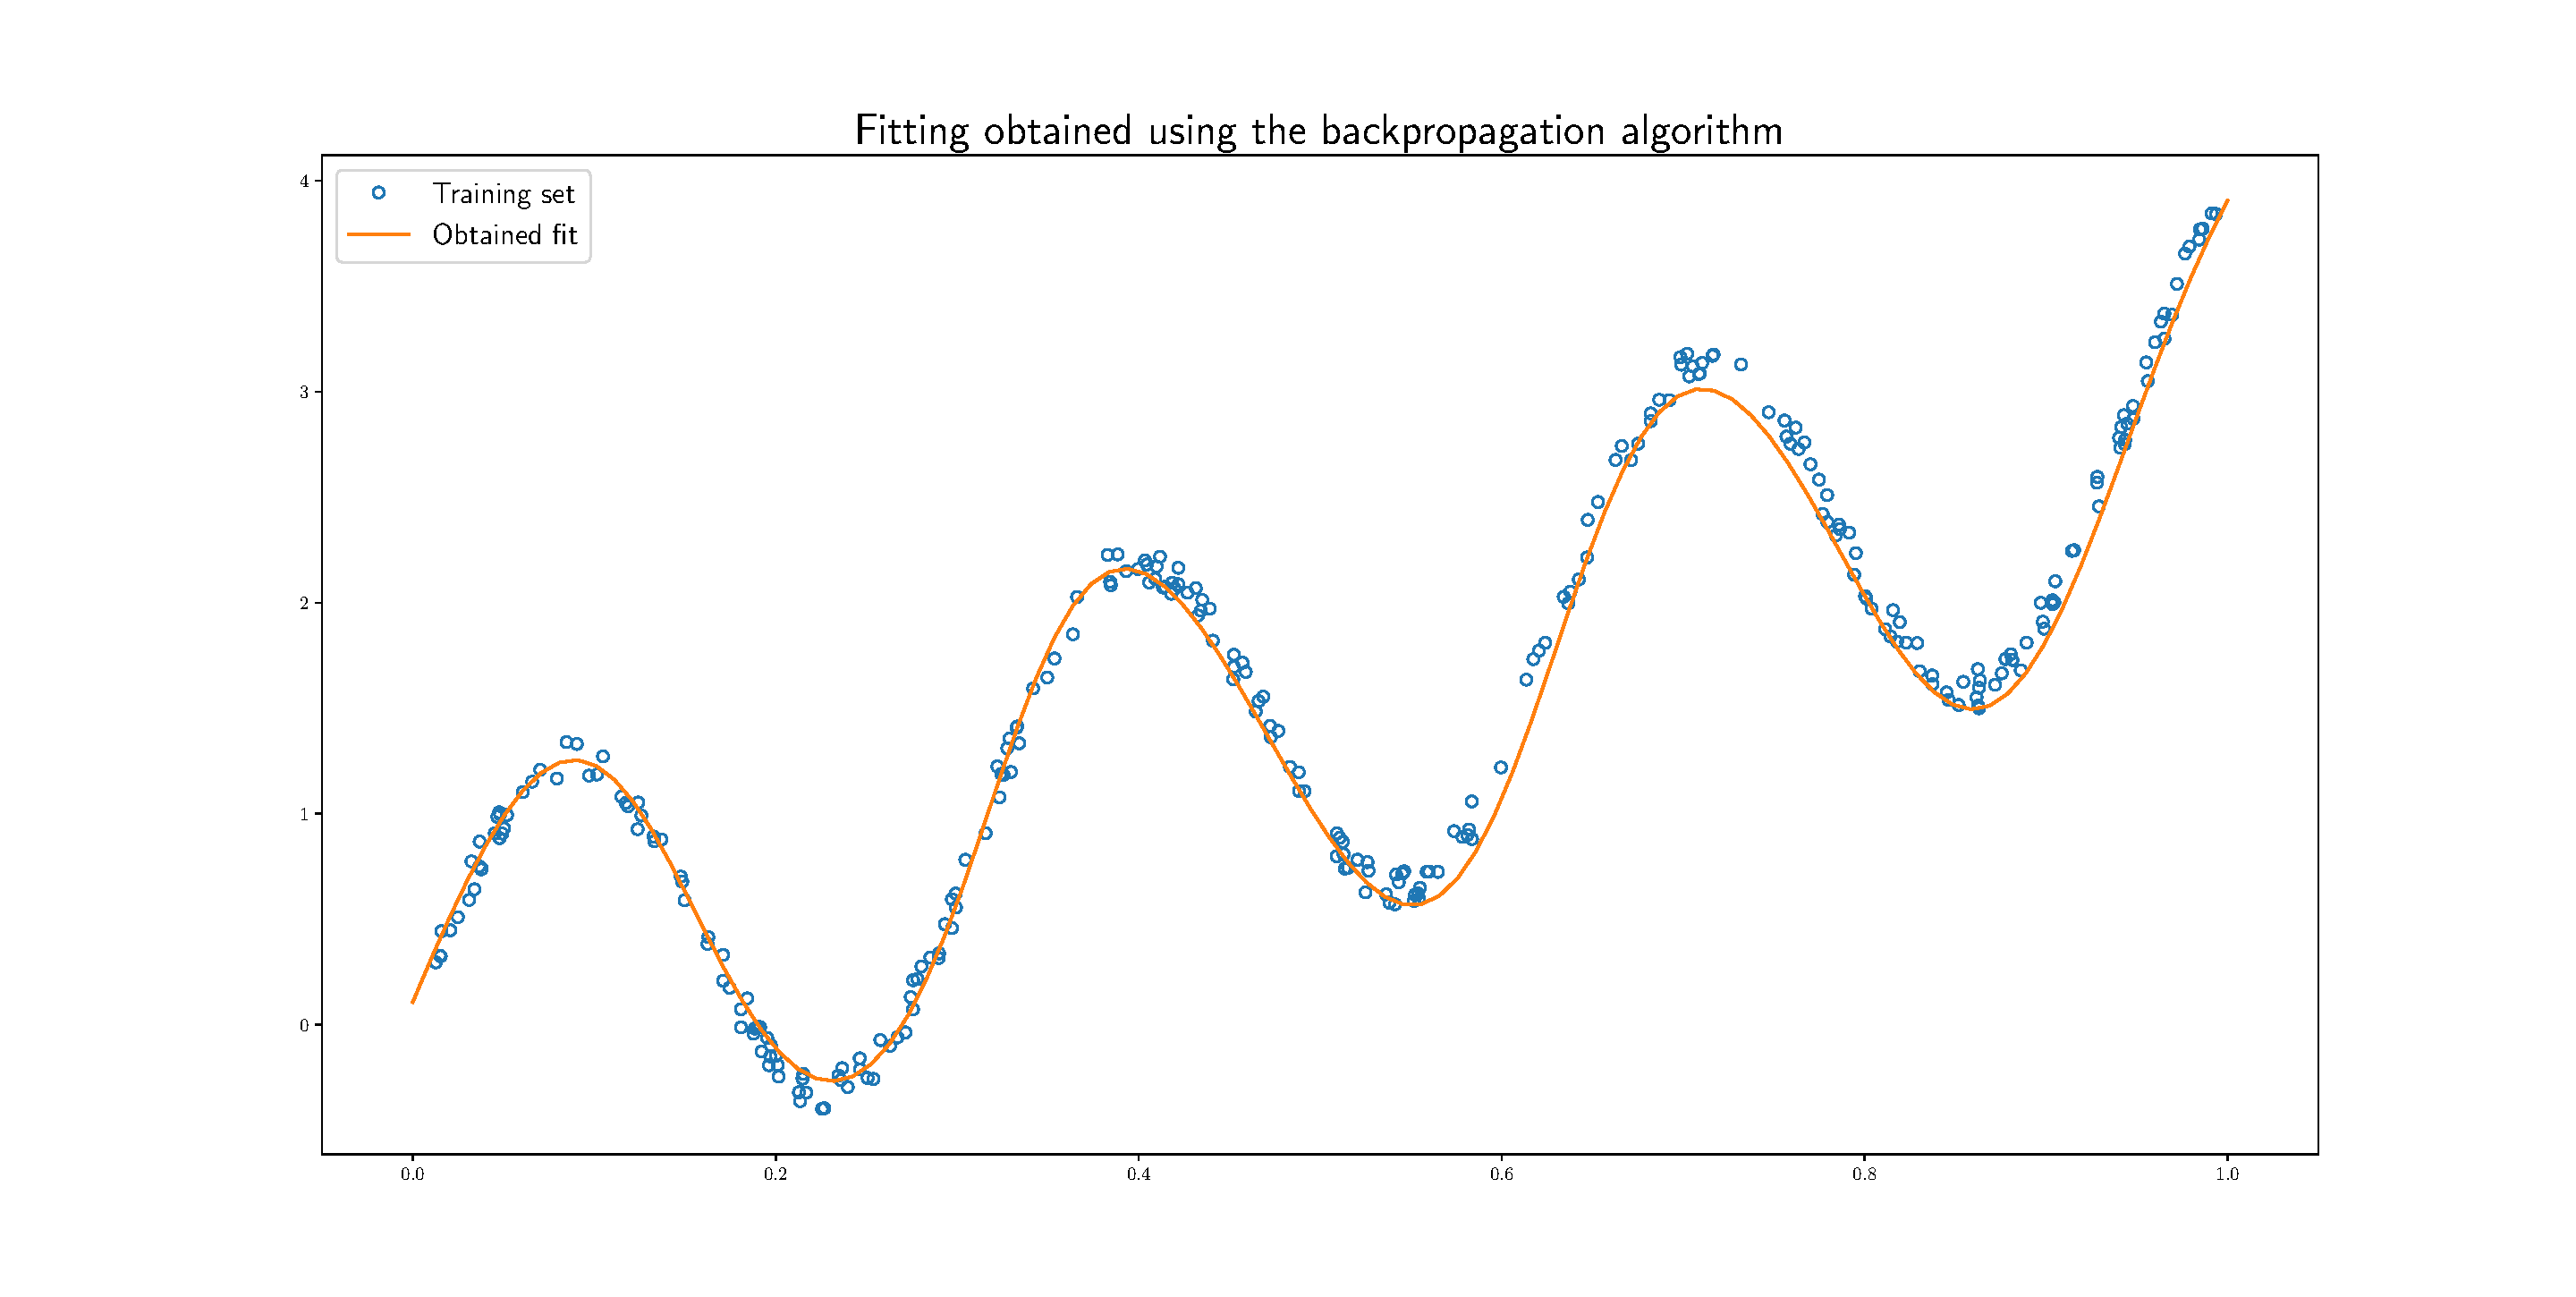
\includegraphics[width=\linewidth]{fit_9.pdf}
\caption{Fitting obtained using backpropagation and $\epsilon = 10^{-9}$}
\label{fit_9}
\end{figure}

\begin{figure}[h]
\centering
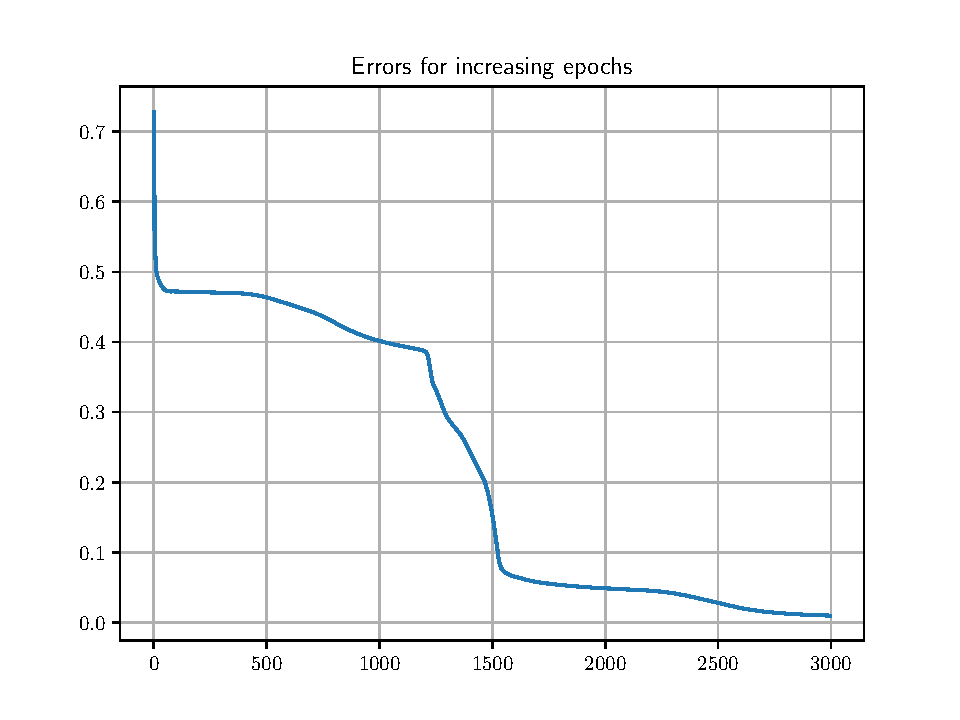
\includegraphics[width=.7\linewidth]{err_9.pdf}
\caption{Error for increasing number of epochs ($\epsilon = 10^{-9}$)}
\label{err_9}
\end{figure}

The obtained fit is close enough to the data points, without exhibiting any major overfitting-related problem (e.g. oscillations in the vicinity of data points). As expected, the major improvements in terms of the reduction of the error function are shown in the first epochs, while the profile becomes almost flat when the number of epochs increases (reduction is limited also by the decreasing value of $\eta$).

\subsection{Complete Python code}

\lstinputlisting[basicstyle=\ttfamily\scriptsize]{hw4.py}

\end{document}